%% LaTeX Beamer presentation template (requires beamer package)
%% see http://latex-beamer.sourceforge.net/
%% idea contributed by H. Turgut Uyar
%% template based on a template by Till Tantau
%% this template is still evolving - it might differ in future releases!

\documentclass[hyperref={pdfpagelabels=false}]{beamer}

\mode<presentation>

\usepackage{graphicx}
\usetheme{isu}
\usepackage{times}
\usepackage{lipsum}
\usepackage{amsmath,amsthm, amssymb, latexsym}
\boldmath
\usepackage[english]{babel}
\usepackage[utf8]{inputenc}
\usepackage{natbib}
\usepackage{textgreek}
\usepackage{mathpartir}
\usepackage{listings}
\bibliographystyle{plainnat}

\DeclareGraphicsExtensions{.pdf,.jpg,.png}
\graphicspath{{figures/}}

\title[Proposal]{
    Axum: Formally Validating Pig Compilation to MapReduce
}
\author[Team Axum: David Johnston and Bijon Bose]{Team Axum: David Johnston and Bijon Bose}
\institute[ISU]{
    Department of Computer Science \linebreak
    Iowa State University\linebreak
    dwtj@iastate.edu\linebreak
    bkbose@iastate.edu
}

\date[COMS 641]{COMS 641: Data Intensive Languages and Systems - Design and Semantics}
%\date{Month X, 20XX}


% If you have a file called "university-logo-filename.xxx", where xxx
% is a graphic format that can be processed by latex or pdflatex,
% resp., then you can add a logo as follows:

%\pgfdeclareimage[height=0.25cm]{logo}{figures/logo}
%\logo{\pgfuseimage{logo}}


\begin{document}
  \begin{frame}[plain]
    \titlepage
  \end{frame}

  \section*{Overview}

\begin{frame}
\begin{itemize}
  \item The Problem
  \begin{itemize}
    \item Correctness of Pig programs depends upon correctness of compilation
          from Pig semantic model to the MapReduce semantic model.
  \end{itemize}

  \item Our Approach
  \begin{itemize}
    \item Coq: Formally model languages, semantics, compilation models; make
          correctness/equivalency proofs.
  \end{itemize}

  \item Evaluation
  \begin{itemize}
    \item Coq: Successfully write correctness proofs.
  \end{itemize}

  \item Benefits
  \begin{itemize}
    \item Formalization of both Pig and MapReduce semantic models can be reused.
    \item More advanced (i.e. optimizing) compilation algorithms can be modeled
          and validated.
  \end{itemize}

\end{itemize}
\end{frame}

  \section{The Problem}
%\begin{frame}
%  \frametitle{Course Rationale: Prevent This Class of Errors}
%  \begin{quote}
%      Language and framework-specific errors, i.e. errors that arise due to
%      incorrect understanding of the semantics of the language and/or framework
%      and its guarantees.
%  \end{quote}
%\end{frame}

\begin{frame}
  \frametitle{The Problem: Program Correctness Depends Upon Compilation
    Correctness}
  \begin{enumerate}
    \item Programs written in sequential, declarative style PigLatin are
    compiled to distributed Hadoop MapReduce jobs.
    \item A Pig program's correctness requires correct compilation.
    \item Correct compilation depends upon a non-trivial mapping from
      properties over Pig semantics to properties over MapReduce semantics
      through the transformation into Logical Plan and Physical Plan.
    \item Our goal is to prove the correctness of this compilation.
  \end{enumerate}
\end{frame}

  \section{Background}

\subsection{Pig-Latin Compilation}
\begin{frame}{Pig Latin Compilation}
\begin{enumerate}
	\item Pig program verification, type checking, schema inference.
	\item Pig program to logical plan (1-1 mapping).
	\item Logical plan to physical plan (map to physical operators).
	\item Physical plan to MapReduce (try to minimize stages).
\end{enumerate}
\end{frame}

%\subsection{MapReduce Execution Model}
%\begin{frame}{MapReduce Execution Model}
%\begin{itemize}
%	\item Map: Produces a stream of data items annotated with keys.
%	\item Local Sort: Orders the data at each machine by key.
%	\item Combiner: Performs partial aggregation on the locally ordered data.
%	\item Shuffle: Redistributes the data to achieve global ordering.
%	\item Merge/Combine: All data received at a particular machine is combined
%          into a single stream in merge stage.
%	\item Reduce: Finally the reduce stage processes the data associated with
%          each key and performs aggregation of the output results.
%\end{itemize}
%\end{frame}
%
%\begin{frame}{MapReduce Execution Model}
%\centerline{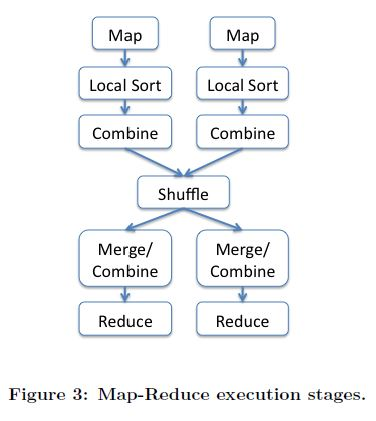
\includegraphics[scale=0.5]{Images/MapReduce_Execution.JPG}}
%\let\thefootnote\relax\footnotetext{\tiny\citet[VLDB][]{gates2009building}}
%\end{frame}

%\subsection{Pig Latin's Logical Plan}
%\begin{frame}{Logical Plan Structure}
%\begin{itemize}
%	\item A Pig Latin program is a sequence of steps, each of which carries out
%          a single transformation.
%	\item Each Pig Latin program is translated to a logical plan
%	\item Pig then translates the logical plan to a physical plan and embeds
%          each physical operator inside a MapReduce stage to arrive at the
%          MapReduce plan.
%\end{itemize}
%\end{frame}

\subsection{PigLatin - Logical Plan}
\begin{frame}{Logical Plan}
\centerline{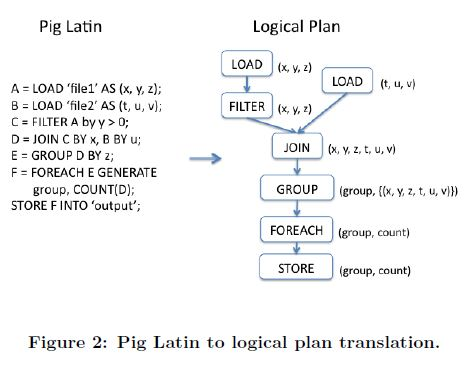
\includegraphics[scale=0.55]{Images/PigLatin.JPG}}
\let\thefootnote\relax\footnotetext{\tiny \citet[VLDB][]{gates2009building}}
\end{frame}

%\subsection{Generating MapReduce Jobs}
%\begin{frame}{Logical-MapReduce}
%\begin{itemize}
%	\item Pig translates the logical plan to a physical plan
%	\item Logical (CO)GROUP operator translates to - local rearrange, global
%          rearrange and package.
%	\item The JOIN is handled either with a COGROUP followed by a FOREACH or
%          fragment replicate join.
%	\item After the physical plan is generated Pig assigns physical operators to
%          Hadoop Stages
%\end{itemize}
%\end{frame}

\subsection{Logical Plan - Physical Plan}
\begin{frame}
\centerline{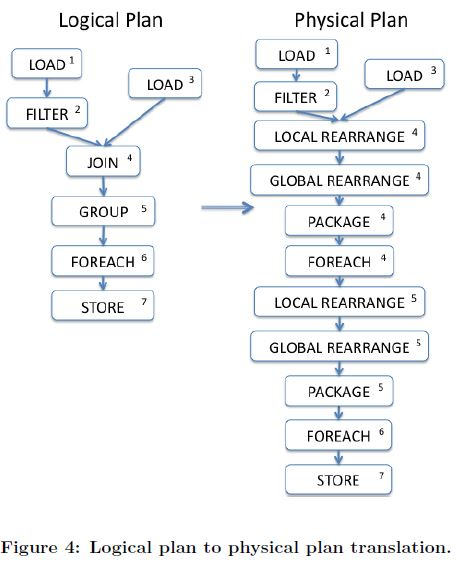
\includegraphics[scale=0.40]{Images/Logical_Physical.JPG} }
\let\thefootnote\relax\footnotetext{\tiny \citet[VLDB][]{gates2009building}}
\end{frame}

\subsection{Physical Plan - Map Reduce}
\begin{frame}
\centerline{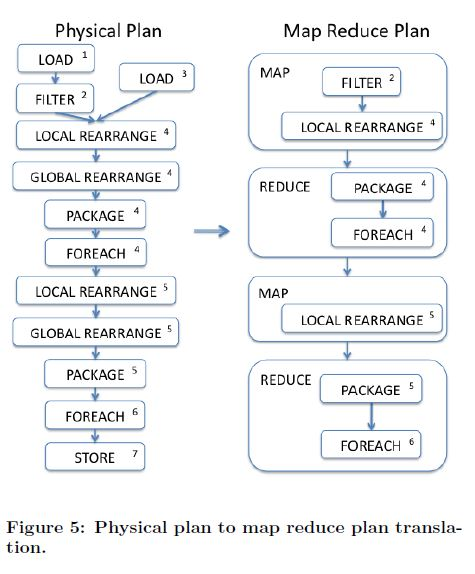
\includegraphics[scale=0.40]{Images/Physical_MapReduce.JPG}}
\let\thefootnote\relax\footnotetext{\tiny \citet[VLDB][]{gates2009building}}
\end{frame}

%\begin{frame}{Pig to MapReduce}
%\begin{itemize}
%	\item Pig compiles programs written in Pig Latin
%	\item Ultimately translates to Map-Reduce tasks
%	\item Pig also operates on local mode running on a single machine without
%          map-reduce
%	\item There lies an equivalence between PigLatin and MapReduce operational
%          semantics
%	\item The equivalence needs to be formalized and correctness needs to be
%          proved
%\end{itemize}
%\end{frame}


%\subsection{Three Main Papers}
%
%\begin{frame}{\citet[VLDB][]{gates2009building}}
%\emph{Building a HighLevel Dataflow System on top of MapReduce: The Pig
%Experience}:
%\begin{itemize}
%	\item This paper outlines the compilation phase of PigLatin programs and how
%          the logical plan of PigLatin is translated to actual Hadoop map-reduce
%          tasks.
%	\item But neither the semantics nor the compilation to map-reduce framework
%          have been formalized with proof of correctness.
%\end{itemize}
%\end{frame}
%
%\begin{frame}{\citet[SEFM]{ono2011using}}
%\emph{Using Coq in Specification and Program Extraction of Hadoop MapReduce
%Applications}
%\begin{itemize}
%    \item Constructed formal model of MapReduce computation in Coq where:
%    \begin{itemize}
%        \item Model user-defined map/reduce as Coq functions
%        \item Application specifications are defined as invariants
%    \end{itemize}
%	\item Constructed formal model of the (previously informally specified)
%          Hadoop libraries
%	\item Using these, they prove the correctness of some example MapReduce
%          applications.
%    \item Future Work: Investigate a more MapReduce applications
%\end{itemize}
%\end{frame}
%
%\begin{frame}{\citet[Journal of Automated Reasoning][]{leroy2009formally}}
%\emph{A formally verified compiler back-end}
%\begin{itemize}
%	\item Compcert: Formally verified compiler from Cminor to PPC assembly.
%    \item Programmed and proven sound using Coq.
%    \item Lots of background on compiler verification.
%\end{itemize}
%\end{frame}

  \section{Our Approach}

\subsection{Core Pig Latin Features}
\begin{frame}{Core Pig Features}
\begin{itemize}
	\item \textbf{Programs specify queries over relations:} Designed to
	concisely facilitate common data transformation tasks.
	\item \textbf{Programs manipulate aggregate non-atomic types:} e.g. bags
	and tuples.
	\item \textbf{Programs use UDFs from environment.}
	\item \textbf{Programs specify data flow via statements:} A sequence of
	statements define dependencies between queries via var assignments and uses.
	\item \textbf{Programs are parallelizable/distributable:} Part of a long
	history in data flow and query-oriented programming.
\end{itemize}
\end{frame}

\subsection{Formalism}
\begin{frame}{Conventions}
\centering
	\begin{flushleft}
		T \quad : a type\newline
		S \quad : a type that satisfies schema type\newline
		c \quad : an integer to denote column offset\newline
		x, y : identifiers\newline
		\textGamma \quad : Context\newline
 		s \quad : a statement\newline
 		q \quad : a term of query form\newline
 		$\vdash$ S c T : column c in Schema S has type T\newline
 		+++ : Schema Concatenation\newline
 		*** : Schema constructed from a pair of types\newline
 		::= : Assignment of statement to ID \newline
 		;; : Sequence of Statements
	\end{flushleft}
\end{frame}

\begin{frame}{Grammar: Terms For Logical Plan}
\centering
%	\begin{flushleft}
%	$ \texttt{tm} := \qquad\qquad\qquad\qquad\qquad\:\: \texttt{Terms}\hfill$\\
%	$ \quad \mid \texttt{t\_filter}\hfill \texttt{Query Filter}\hfill$\\
%   	$ \quad \mid \texttt{t\_foreach} \hfill \texttt{Query ForEach}\hfill$\\
%    $ \quad \mid \texttt{t\_group} \hfill \texttt{Query Group}\hfill$\\
%    $ \quad \mid \texttt{t\_join} \hfill \texttt{Query Join}\hfill$\\
%    $ \quad \mid \texttt{t\_load} \hfill \quad\quad\:\: \texttt{Load Statement}\hfill$\\
%   	$ \quad \mid \texttt{t\_assign} \hfill \qquad\qquad\quad \texttt{Assignment Statement}\hfill$\\
%    $ \quad \mid \texttt{t\_seq} \hfill \qquad\qquad\qquad\quad\quad \texttt{Sequence of Statements}\hfill$\\
%    $ \quad \mid \texttt{t\_store} \hfill \quad\quad\:\: \texttt{Store Statement}\hfill$\\
%	\end{flushleft}
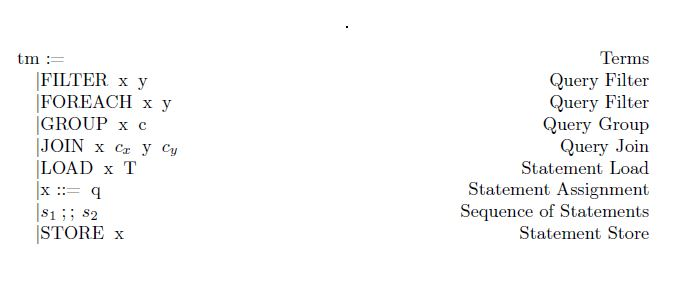
\includegraphics[scale=0.6]{Images/Grammar/Terms.JPG}
\end{frame}


\begin{frame}{Grammar: Terms For Physical Plan}
\centering
%	\begin{flushleft}
%	$ \texttt{tm} := \qquad\qquad\qquad\qquad\qquad\:\: \texttt{Terms}\hfill$\\
%	$ \quad \mid \texttt{t\_filter}\hfill \texttt{Query Filter}\hfill$\\
%   	$ \quad \mid \texttt{t\_foreach} \hfill \texttt{Query ForEach}\hfill$\\
%    $ \quad \mid \texttt{t\_lrearrange} \hfill \texttt{Query Local ReArrange}\hfill$\\
%    $ \quad \mid \texttt{t\_grearrange} \hfill \texttt{Query Global ReArrange}\hfill$\\
%    $ \quad \mid \texttt{t\_package} \hfill \texttt{Query Package}\hfill$\\
%    $ \quad \mid \texttt{t\_load} \hfill \quad\quad\:\: \texttt{Load Statement}\hfill$\\
%   	$ \quad \mid \texttt{t\_assign} \hfill \qquad\qquad\quad \texttt{Assignment Statement}\hfill$\\
%    $ \quad \mid \texttt{t\_seq} \hfill \qquad\qquad\qquad\quad\quad \texttt{Sequence of Statements}\hfill$\\
%    $ \quad \mid \texttt{t\_store} \hfill \quad\quad\:\: \texttt{Store Statement}\hfill$\\
%	\end{flushleft}
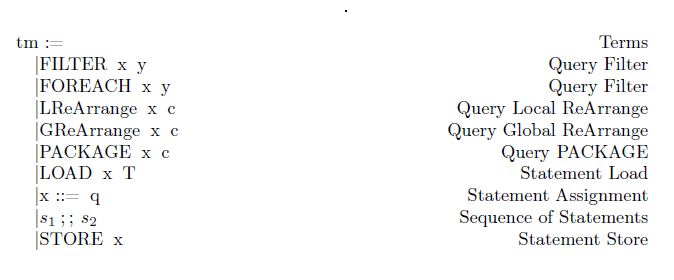
\includegraphics[scale=0.6]{Images/Grammar/Terms_Physical.JPG}
\end{frame}

\begin{frame}{Grammar: Schema Types}
\centering
%	\begin{flushleft}
%	$ schema := \hfill \quad Schema \:Types\hfill$\\
%	$ \quad \mid \texttt{STNil}\hfill \texttt{{Unit Type}}\hfill$\\
%   	$ \quad \mid \texttt{STyPair} \hfill \texttt{Tuple of Column and Schema}\hfill$\\
%
%	$ \texttt{schema} := \hfill \quad\texttt{Schema Types}\hfill$\\
%	$ \quad \mid \texttt{STNil}\hfill \texttt{{Unit Type}}\hfill$\\
%   	$ \quad \mid \texttt{STyPair} \hfill \texttt{Tuple of Column and Schema}\hfill$\\
%
%	\end{flushleft}
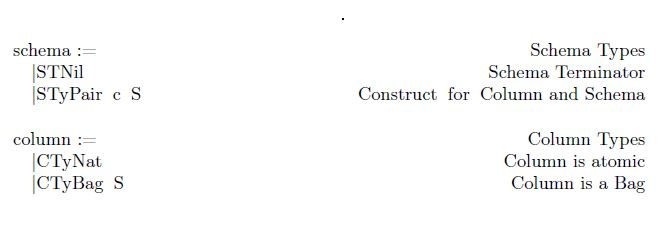
\includegraphics[scale=0.6]{Images/Grammar/Schema.JPG}
\end{frame}

\begin{frame}{Grammar: Types}
\centering
%	\begin{flushleft}
%	$ \texttt{ty} := \qquad\qquad\qquad\qquad\quad\quad\:\: \texttt{Types}\hfill$\\
%	$ \:\:\: \mid \texttt{TUnit}\hfill \texttt{Unit Type}\hfill$\\
%   	$ \:\:\: \mid \texttt{TFn} \hfill\qquad\quad\:\: \texttt{Function Type}\hfill$\\
%    $ \:\:\: \mid \texttt{TPred} \hfill\qquad\quad \texttt{Predicate Type}\hfill$\\
%    $ \:\:\: \mid \texttt{TNil} \hfill \qquad\qquad\qquad\qquad\:\:\: \texttt{Schema Tuple Terminator}\hfill$\\
%    $ \:\:\: \mid \texttt{TCons} \hfill \qquad\qquad\qquad\quad\:\: \texttt{Schema Tuple Extension}\hfill$\\
%   	$ \:\:\: \mid \texttt{TInt} \hfill \qquad\qquad\qquad\qquad\quad \texttt{Atomic Schema Attribute}\hfill$\\
%    $ \:\:\: \mid \texttt{TBag} \hfill \quad\qquad\qquad\qquad\qquad\: \texttt{Compound Schema Attribute}\hfill$\\
%	\end{flushleft}
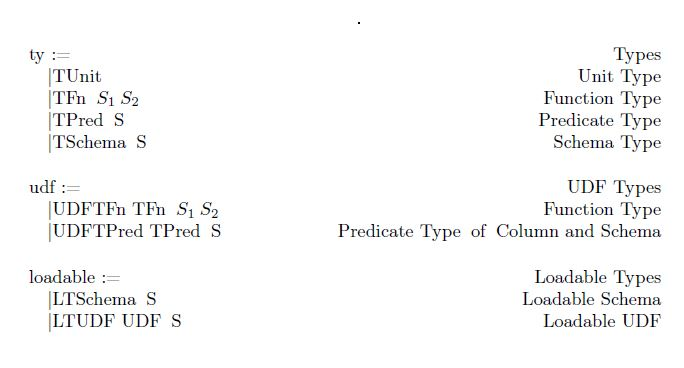
\includegraphics[scale=0.6]{Images/Grammar/Types.JPG}
\end{frame}

\subsection{Typing Rules for Logical Plan}
\begin{frame}{Typing Rules: Queries}
\centering
%	\begin{mathpar}
%		\inferrule* [Right=\texttt{T\_Filter}]
%          		{\Gamma \vdash \texttt{x = S} \\ \texttt{schema \:S} \\
%          		\Gamma \vdash \texttt{y = Pred \:S}}
%          		{\Gamma \vdash \texttt{FILTER \:x, y} \in \texttt{S} }
%		\hva \and
%		\inferrule* [Right={\textbf{T\_ForEach}}]
%          		{schema \:S_1 \\ schema \:S_2 \\\\
%				\Gamma \vdash x = S_1 \\ \Gamma \vdash y = Fn\: S_1\:S_2}
%				{\Gamma \vdash FOREACH \:x\:y \in S }
%	\end{mathpar}
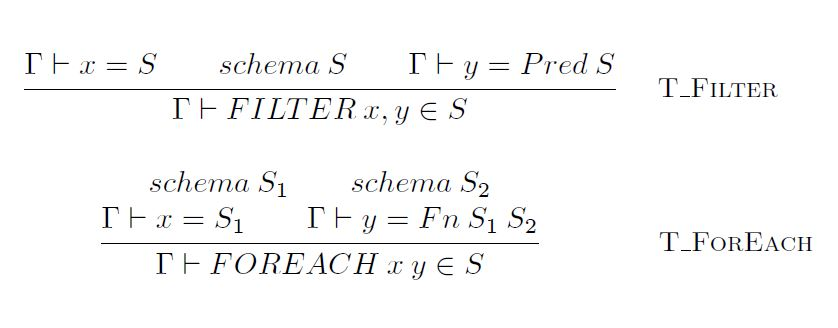
\includegraphics[scale=0.4]{Images/TypingRules/FilterForeach.JPG}
\end{frame}

\begin{frame}{Typing Rules: Queries(continued...)}
\centering
%	\begin{mathpar}
%		\inferrule* [Right=\textbf{T\_Group}]
%          		{\Gamma \vdash x = S \\\\
%          		schema \:S \\ schema \:S' \\\\
%          		schema\_column\_has\_type \:S \:c \\\\
%          		S' = TInt ::: (TBag \:S)}
%          		{\Gamma \vdash GROUP \:x \:c \in S' }
%	\end{mathpar}
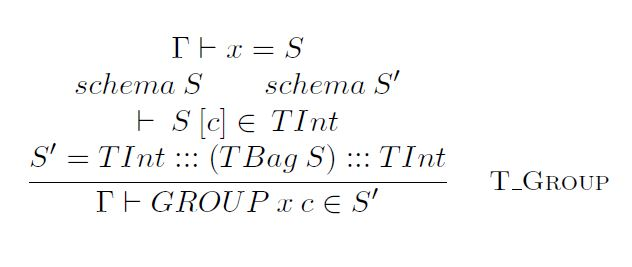
\includegraphics[scale=0.4]{Images/TypingRules/Group.JPG}
\end{frame}

\begin{frame}{Typing Rules: Queries(continued...)}
\centering
%	\begin{mathpar}
%		\inferrule* [Right=\textbf{T\_Join}]
%          		{\Gamma \vdash x = S_1 \\ \Gamma \vdash y =  S_2 \\\\
%          		schema\:S_1 \\ schema \:S_2 \\\\
%		 		schema\_column\_has\_type \:S_1 \:c_x \\\\
%		 		schema\_column\_has\_type \:S_2 \:c_y \\\\
%		 		concatenated\_schema \:S_1\:S_2\:S_3}
%		 		{\Gamma \vdash JOIN \:x \:c_x \:y \:c_y \in S_3 }
%	\end{mathpar}

\includegraphics[scale=0.4]{Images/TypingRules/Join.JPG}
\end{frame}

\begin{frame}{Typing Rules: Statements}
\centering
%	\begin{mathpar}
%		\inferrule* [Right=\textbf{T\_Load}]
%          		{\Gamma \vdash x = None \\ loadable\_ty\: T}
%          		{\Gamma \vdash LOAD \:x\:T \in TUnit }
%		\hva \and
%		\inferrule* [Right=\textbf{T\_Assign}]
%          		{\Gamma \vdash x = None \\ \Gamma \vdash q = S \\schema \:S}
%          		{\Gamma \vdash ASSIGN \:x \:q \in TUnit }
%		\hva \and
%		\inferrule* [Right=\textbf{T\_Store}]
%				{\Gamma \vdash x = S \\ schema \:S}
%				{\Gamma \vdash STORE \:x \in TUnit }
%	\end{mathpar}
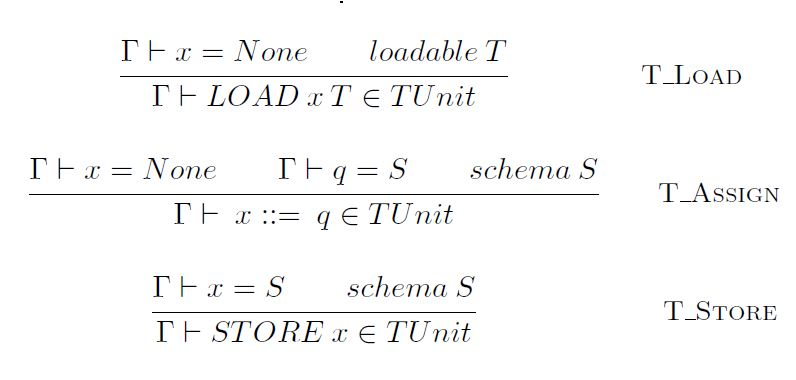
\includegraphics[scale=0.4]{Images/TypingRules/Load_Assign_Store.JPG}
\end{frame}

\begin{frame}{Typing Rules: Statements (continued...)}
\centering
%	\begin{mathpar}
%		\inferrule* [Right=\textbf{T\_SeqLoad}]
%          		{s_1 = LOAD \:x \:T \\ \Gamma \vdash s_1 \in TUnit \\\\
%          		\Gamma, x:T \vdash s_2 \in TUnit }
%          		{\Gamma \vdash SEQ \:s_1 \:s_2 \in TUnit }
%
%		\hva \and
%		\inferrule* [Right=\textbf{T\_SeqAssign}]
%          		{s_1 = ASSIGN \:x \:q \\\\
%          		\Gamma \vdash q = S \\ schema \:S \\\\
%          		\Gamma \vdash s_1 \in TUnit \\ \Gamma, x:S \vdash s_2 \in TUnit}
%          		{\Gamma \vdash SEQ \:s_1 \:s_2 \in TUnit }
%	\end{mathpar}
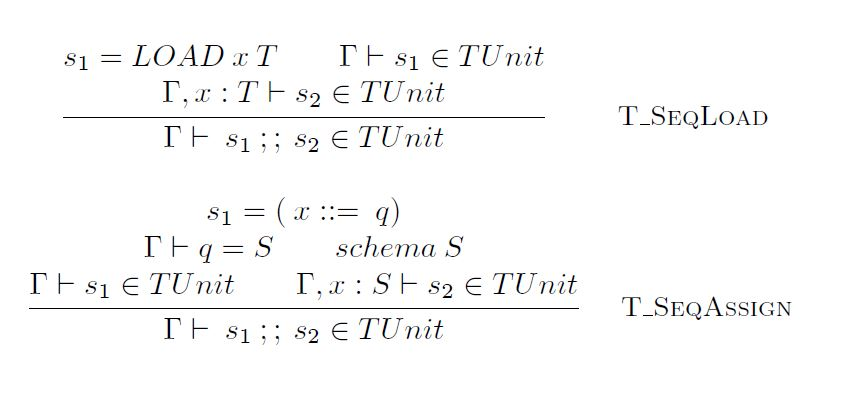
\includegraphics[scale=0.4]{Images/TypingRules/SEQ1.JPG}
\end{frame}

\begin{frame}{Typing Rules: Statements (continued...)}
\centering
%	\begin{mathpar}
%		\inferrule* [Right= \textbf{T\_SeqStore}]
%          	{s_1 = STORE \:x \\\\
%          	\Gamma \vdash x = S \\ schema \:S  \\\\
%			\Gamma \vdash s_1 \in TUnit \\ \Gamma \vdash s_2 \in TUnit }
%			{\Gamma \vdash SEQ \:s_1 \:s_2 \in TUnit }
%	\end{mathpar}

\includegraphics[scale=0.4]{Images/TypingRules/SEQ2.JPG}
\end{frame}

\subsection{Typing Rules for Physical Plan}
\begin{frame}{Typing Rules: Queries}
\centering
%	\begin{mathpar}
%		\inferrule* [Right=\texttt{T\_LReArrange}]
%          		{\Gamma \vdash \texttt{x = S} \\ \texttt{schema \:S} \\\\
%          		schema\_column\_has\_type \:S \:c}
%          		{\Gamma \vdash \texttt{LReArrange \:x c} \in \texttt{S} }\\
%		\inferrule* [Right=\texttt{T\_GReArrange}]
%          		{\Gamma \vdash \texttt{x = S} \\ \texttt{schema \:S} \\\\
%          		schema\_column\_has\_type \:S \:c}
%          		{\Gamma \vdash \texttt{GReArrange \:x c} \in \texttt{S} }
%	\end{mathpar}
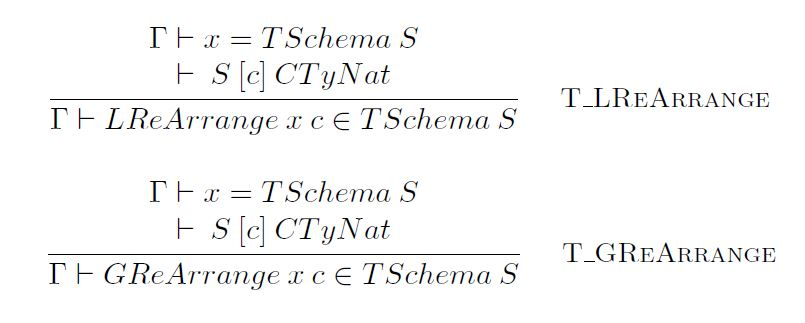
\includegraphics[scale=0.4]{Images/TypingRules/ReArrange.JPG}
\end{frame}

\begin{frame}{Queries(continued...)}
\centering
%	\begin{mathpar}
%		\inferrule* [Right=\texttt{T\_Package}]
%          		{\Gamma \vdash \texttt{x = S} \\ \texttt{schema \:S} \\\\
%          		schema\_column\_has\_type \:S \:c \\\\
%				S' = TInt ::: (TBag S) \\ \texttt{schema \:S'}}
%          		{\Gamma \vdash \texttt{Package \:x c} \in \texttt{S'} }
%	\end{mathpar}

\includegraphics[scale=0.4]{Images/TypingRules/Package.JPG}
\end{frame}


\subsection{Semantics via Specification Relations}

\begin{frame}{Semantics: Representing Relations with multiset}
\centering
  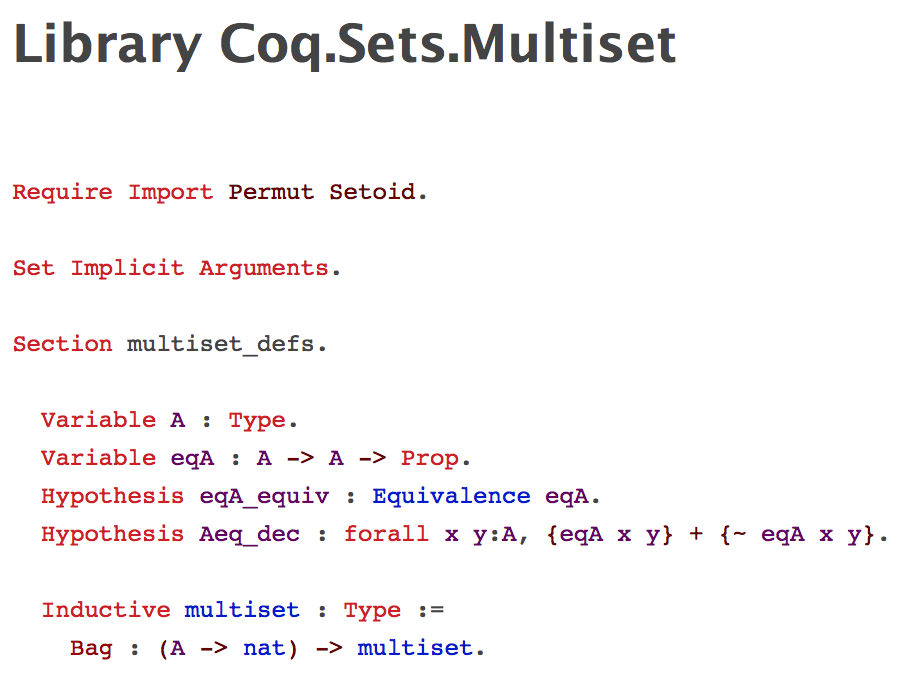
\includegraphics[scale=0.5]{CoqIDE/Semantics/Multisets.png}
\end{frame}

\begin{frame}{Semantics: Representing Relations with multiset}
\centering
  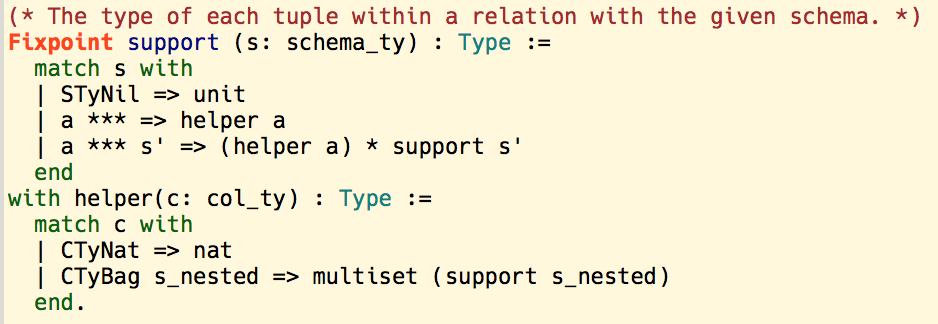
\includegraphics[scale=0.55]{CoqIDE/Semantics/support.png}
	\\[3ex]
  
\includegraphics[scale=0.55]{CoqIDE/Semantics/relation.png}
\end{frame}

\begin{frame}{Semantics: Four Key Specification Properties}
\centering
  \begin{enumerate}
  \item \texttt{filtered}
	\item \texttt{mapped}
	\item \texttt{grouped}
	\item \texttt{joined}
  \end{enumerate}
\end{frame}

\begin{frame}{Semantics: The \texttt{filtered} Specification}
\centering
  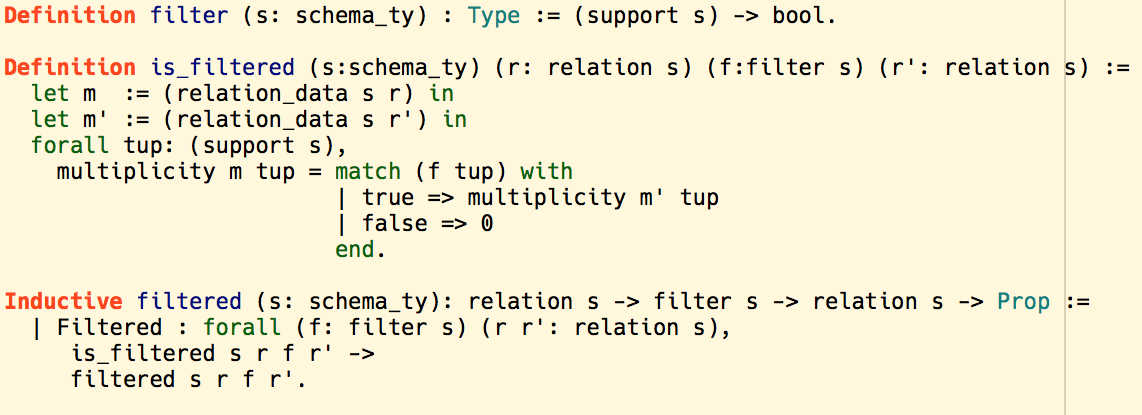
\includegraphics[scale=0.55]{CoqIDE/Semantics/filtered.png}
\end{frame}

\begin{frame}{Semantics: The \texttt{mapped} Specification}
\centering
  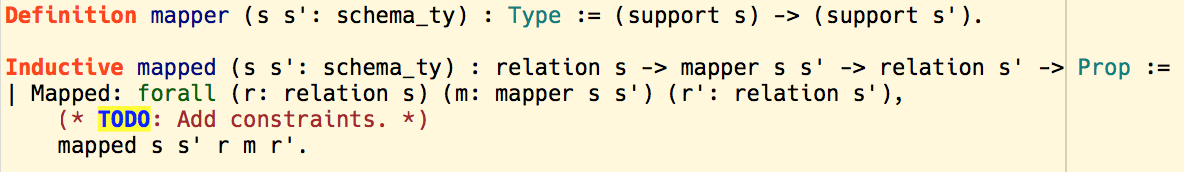
\includegraphics[scale=0.55]{CoqIDE/Semantics/mapped.png}
\end{frame}

\begin{frame}{Semantics: The \texttt{grouped} Specification}
\centering
  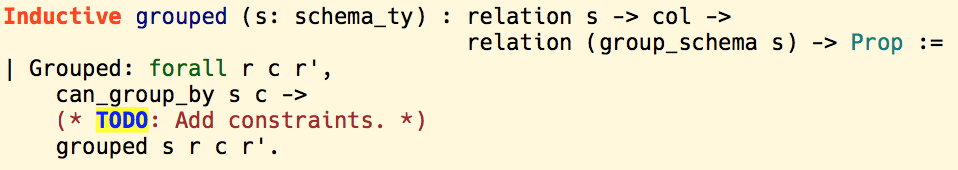
\includegraphics[scale=0.65]{CoqIDE/Semantics/grouped.png}
\end{frame}

\begin{frame}{Semantics: The \texttt{joined} Specification}
\centering
  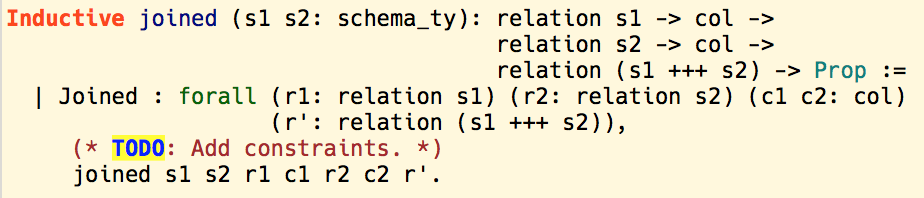
\includegraphics[scale=0.65]{CoqIDE/Semantics/joined.png}
\end{frame}

  \section{Challenges}

\begin{frame}{Challenges}
To challenges in the formalization for Pig Latin are -
\begin{itemize}
	\item To identify and differentiate between the different phases of PigLatin
	\item Develop core semantics for each phases while maintaining the core features of Pig Latin
	\item How to represent the equivalence between different phases
\end{itemize}
\end{frame}

  %\section*{}

\subsection{Pig Latin}
\begin{frame}
  \begin{itemize}
    \item \citet[SIGMOD][]{olston2008pig} \\
          \emph{Pig-Latin: A not-so-foreign language for data processing}
    \item \citet[VLDB][]{gates2009building} \\
          \emph{Building a high-level dataflow system on top of Map-Reduce: the
          Pig experience}
    \item \citet[TASS][]{zhang2013performance} \\
          \emph{Performance Modeling and Optimization of Deadline-Driven Pig
          Programs}
  \end{itemize}
\end{frame}

\subsection{MapReduce Model}
\begin{frame}
  \begin{itemize}
    \item \citet[CACM][]{dean2004mapreduce} \\
          \emph{MapReduce: Simplified Data Processing on Large Clusters}
    \item \citet[SIGMOD][]{yang2007map} \\
          \emph{Map-reduce-merge: Simplified relational data processing on large
          clusters}
    \item \citet[ICSE][]{xiao2014nondeterminism} \\
          \emph{Nondeterminism in mapreduce considered harmful? ...}
    \item \citet[ASPLOS][]{leesatapornwongsa2016taxdc} \\
          \emph{TaxDC: A Taxonomy of Non-Deterministic Concurrency Bugs in
          Datacenter Distributed Systems}
  \end{itemize}
\end{frame}

\subsection{Formalisms and Correct Usage of MapReduce}
\begin{frame}[allowframebreaks]
  \begin{itemize}
    \item \citet[Science of Computer Programming][]{lammel2008google} \\
          \emph{Google's MapReduce programming model--Revisited}
    \item \citet[ABZ][]{pereverzeva2014formal} \\
          \emph{Formal Derivation of Distributed MapReduce}
    \item \citet[TACAS][]{chen2015commutativity} \\
          \emph{Commutativity of Reducers}
    \item \citet[Concurrency and Computation][]{dorre2015modeling} \\
          \emph{Modeling and optimizing MapReduce programs}
    %\item \citet[ECBS][]{yang2010formalizing} \\
    %      \emph{Formalizing MapReduce with CSP}
    \item \citet[SEFM][]{ono2011using} \\
          \emph{Using Coq in Specification and Program Extraction of Hadoop
          MapReduce Applications}
  \end{itemize}
\end{frame}

  \section*{}

%\textsc{\textsc{\textsc{\begin{frame}{Future Work}
  %\begin{itemize}
    %\item % TODO Talk about future work/limitations here
  %\end{itemize}
%\end{frame}


%\begin{frame}{Conclusion}
% TODO copy/paste overview here (from intro.tex)
%\end{frame}}


\begin{frame}
\begin{beamercolorbox}[center]{white}
  {\Large Questions?}

  \vspace{2em}\hfill

  \url{https://github.com/isu-cs641s16-axum}
\end{beamercolorbox}
\end{frame}


  \begin{frame}[allowframebreaks]
    \bibliography{refs}{}
  \end{frame}
  \appendix

% make sure you have a blank slide in case you accidentally go past your conclusion
\begin{frame}
  % Nothing here.
\end{frame}


% these slides are to help answer potential questions and generally arent shown
% unless needed or there is extra time
\begin{frame}[plain]{Hidden Slide 1}
\end{frame}

\begin{frame}[plain]{Hidden Slide 2}
\end{frame}

\end{document}
